%%
% !TeX program = lualatex
%%

\documentclass[
    DIV=calc,
    IMRAD=false,
	ngerman,
	accentcolor=1c,% Farbe für Hervorhebungen auf Basis der Deklarationen in den Corporate Design Richtlinien
%	logofile=example-image, %Falls die Logo Dateien nicht vorliegen
	marginpar=false,
	identbarcolor=1c,
	]{tudapub}
\usepackage[T1]{fontenc}

\usepackage[english, main=ngerman]{babel}
\usepackage[babel]{csquotes}

\usepackage{hologo}

\usepackage{floatrow}
%\usepackage{subfig}
\newfloatcommand{capbtabbox}{table}[][\FBwidth+5cm]
\usepackage{blindtext}
\usepackage{colortbl}
\usepackage{ifthen}

%\usepackage[demo]{graphicx}
\usepackage{caption}
\usepackage[skip=0cm,list=true,labelfont=it]{subcaption}

\newcommand{\unit}[1]{{\rm\,#1}}

\newboolean{sensorsDetailed}
\setboolean{sensorsDetailed}{true}


\begin{document}

%Zusätzliche Metadaten für PDF/A. In diesem Fall notwendig, weil Titel ein Makro enthält.
\Metadata{
	author=NeXT,
	title=Space Workshop Dokumentation,
	%subject=Basisdokumentation und Template zur Nutzung der tudapub-Dokumentenkasse,
	%date=2019-04-29,
	%keywords=TU Darmstadt \sep Corporate Design \sep LaTeX
}




\title{Space Workshop\newline L\"osungshinweise}
\subtitle{NeXT Generation on Campus}
%\author{Marei Peischl\thanks{pei\TeX{} \TeX{}nical Solutions}\and der \TeX-Löwe}
\date{}
\titleimage{
%	%Folgende Box kann selbstverständlich durch ein mit \includegraphics geladenes Bild ersetzt werden.
\bigskip
\bigskip
\bigskip
\bigskip
\bigskip
\bigskip
\bigskip
\bigskip
\bigskip
\bigskip
\bigskip
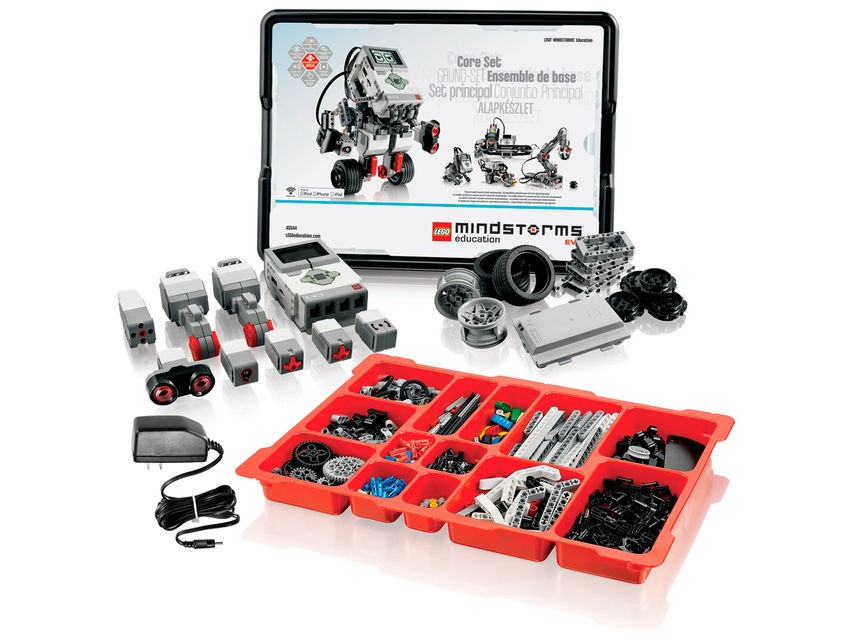
\includegraphics[width=\textwidth]{images/title.jpg}
	%\color{black!30}\rule{\width}{\height}
}


%Varianten der Infoboxen
\addTitleBox{\includegraphics[width=\linewidth]{../../ist_logo.pdf}}
%\addTitleBoxLogo{example-image}
%\addTitleBoxLogo*{\includegraphics[width=.3\linewidth]{example-image}}



\maketitle


\newpage
\section{Allgemein}
Zur Bearbeitung der einzelnen Space-Aufgaben gibt es keine richtige Musterl\"osung, dennoch m\"ochten wir hier ein paar allgemeine Hinweise und Vorschl\"age geben. Prinzipiell gilt, dass der Programmcode unterschiedlich \glqq{}sch\"on\grqq und kurz geschrieben werden kann, es aber viele Wege zum Ziel gibt.

\section{Basis}
In der Basis gibt es Markierungen f\"ur zwei Startpl\"atze, sodass man immer von der gleichen Stelle starten kann, sodass der Code entsprechend angepasst werden kann.\newline
Wenn der Roboter jedoch leicht versetzt startet, kann es zu Problemen kommen. F\"ur dieses Problem gibt es wei\ss{}e Streifen an denen sich der Roboter orientieren kann um sich entsprechend auszurichten.

\section{Satellitensch\"ussel}
Diese Station ist eine der einfacheren Station, hier f\"ahrt der Roboter lediglich dagegen und startet. Doch auch hier kann man mit Sensoren arbeiten um die Ausf\"uhrung flexibler zu gestalten. Hier kann beispielsweise mit dem Ultraschallsensor die Distanz zum Hindernis gemessen werden um die Geschwindigkeit auf dem Weg anzupassen. Oder der Roboter pr\"uft mit dem Ber\"uhrungssensor, ob er am Ziel angelangt ist um dann zu stoppen und umzukehren.

\section{Weltraumschrott}
Bei dieser Aufgabe ist es besonders wichtig, eine mechanisch gute Konstruktion zu bauen um alle Steine einsammeln zu k\"onnen.

\section{Marsroboter}
Um den Marsroboter zu retten ist es wichtig, die richtige Distanz zu fahren. Hierbei kann mit dem Farbsensor gepr\"uft werden, wann die Stufe der Rampe erreicht wird um dann die restliche Strecke absch\"atzen zu k\"onnen. F\"ur das Greifen des Roboters ist es sinnvoll, eine Konstruktion zu bauen, die bei Erreichen des Zielobjektes heruntergeklappt wird, damit der Roboter aus seiner misslichen Lage gezogen werden kann.

\section{Solarpanel}
Auch vor dem Solarpanel gibt es farbliche Streifen an denen man den Roboter ausrichten kann, damit er mit der notwendigen Pr\"azision auf das Panel zuf\"ahrt. Zur Drehung ist der mittlere Motor sinnvoll der flexibel vorne angebracht werden kann.

\section{Crew-Mitglieder}
Auf \"ahnlich Weise kann man den Roboter auch vor den Crew-Mitgliedern ausrichten, damit der Roboter erfolgreich den richtigen Astronauten retten kann.

\section{Satellit}
F\"ur den Satelliten befindet sich eine Markierung auf dem Spielplan. Auch diese kann mit den Farbsensoren erfasst werden um den Satelliten dort pr\"azise abzusetzen.

\section{Rakete}
Der Abschluss der Space-Mission ist der Start der Rakete. Hierbei muss mit starker Kraft auf die Platte hinter der Rakete gedr\"uckt werden. Hierbei liegt die Schwierigkeit diese gro\"ss{}e Kraft zu erreichen. Zum einen ist zu beachten, dass der gro\ss{}e Motor mehr Kraft hat, sich aber langsamer bewegt als der mittlere Motor. Ebenso kann mit einem l\"angeren Arm am Roboter gearbeitet werden sowie mit einer m\"oglichst gro\ss{}en Masse am Ende des Arms um die Kraft zu vergr\"o\ss{}ern.

\bigskip \bigskip \bigskip

\tiny Das Bild ist der Internetseite des offiziellen Lego-Onlineshops lego.com entnommen. Die Urheberrechte befinden sich im Besitz der LEGO Gruppe, diese Anleitung ist unabh"angig und wurde von der LEGO Gruppe weder autorisiert noch gesponsert.
\cfoot{\textcolor{lightgray} \today}




\end{document}
